\documentclass[11pt, a4paper]{article}
\usepackage[dutch]{babel}
\usepackage{newpxtext}
\usepackage{graphicx}

\begin{document}
\title{User stories voor de Quizmaster}
\date{\today}
\author{Huub van Thienen}
\maketitle
\begin{abstract}
In dit document worden de user stories beschreven van het systeem dat de MIW2.0 cursisten in het eerste project gaan bouwen.
\end{abstract}

\section{Algemeen}

In dit hoofdstuk worden de user stories beschreven die voor alle rollen gelden. Ook is er een overzicht van de rollen.

\subsection{Objecten}
Bij de beschrijving van het Quizmaster systeem worden een aantal objecten gebruikt die hier worden beschreven.

\paragraph{Gebruiker} Een gebruiker is iemand die gebruik mag maken van het systeem. 
De Quizmaster legt van iedere gebruiker de naam, het password en de rol vast. 
Gebruikers krijgen toegang tot de Quizmaster door hun naam en password in te voeren in het login scherm.

\paragraph{Cursus} Een cursus heeft een naam en een co\"ordinator.
Een cursus heeft nul of meer groepen die deze cursus volgen.
Bij een cursus horen nul of meer quizes.

\paragraph{Groep} Een groep is een aantal studenten die een bepaalde cursus volgt, daarom heeft iedere groep een cursus.
Een student die meerdere cursussen volgt wordt voor iedere cursus in een groep ingedeeld, het is dus niet zo dat een student voor het hele stdiejaar in dezelfde groep zit.
Iedere groep heeft een naam en een docent.
Een coordinator (van de cursus bij deze groep of van een andere cursus) kan ook docent van een groep zijn.

\paragraph{Quiz}
Een quiz hoort bij een cursus.
Een quiz bestaat uit \'e\'en of meer multiple-choicevragen.
Iedere vraag heeft twee of meer antwoorden.

\subsection{Rollen}

\paragraph{Student} Een \emph{student} maakt alle toetsen die voor een cursus vereist zijn.

\paragraph{Docent} Een \emph{docent} gebruikt het systeem om de voortgang van de studenten in zijn klas te bewaken.
Daartoe vraagt hij overzichten op van de studenten en hun prestaties tot nu toe.

\paragraph{Co\"ordinator} Een \emph{co"ordinator} is verantwoordelijk voor het beheer van de toetsen.
Zij voert vragen in (met de antwoorden natuurlijk!) en bepaalt de succesdefinitie. Iedere co\"ordinator is ook docent en kan dus ook alle taken die bij de docentrol horen uitvoeren.

\paragraph{Onderwijsadminstratie} Een \emph{administrator} maakt klassen, deelt cursisten in en wijst een leraar toe aan die klas.
Ook bepaalt hij wie er co"ordinator is van die cursus.

\paragraph{Technisch beheerder} Een \emph{systeembeheerder} is verantwoordelijk voor het functioneren van het systeem.
Hij maakt gebruikers aan met een naam en een password.
Van iedere gebruiker legt hij de rol vast.

\section{User stories}

\subsection{Algemeen}

\paragraph{Inloggen}
Als gebruiker wil ik in het systeem kunnen inloggen zodat ik de functies die bij mijn rol horen kan uitvoeren. (scherm login.fxml, loginFailed.fxml).

\paragraph{Taakselectie}
Als gebruiker wil ik na het inloggen een overzicht vand de mogelijke taken krijgen zodat ik daar een keuze uit kan maken. (scherm welcomeScene.fxml).
Bij deze keuze wil ik alleen de taken aangeboden krijgen die bij mijn rol passen.

\subsection{User stories voor de rol Student}

\paragraph{In- en Uitschrijven}
Als student wil ik mij voor een cursus kunnen in- of schrijven zodat ik de bij quizes van die cursus kan maken.
Bij de inschrijving wil ik mij voor meerdere cursussen tegelijk kunnen inschrijven.

\paragraph{Opmerking}
Voor het in- en uitschrijven wordt hetzelfde scherm gebruikt. Dit scherm bevat twee lijsten, links de lijst met cursussen waarvoor de student nog niet is ingeschreven, rechts de lijst met cursussen waarvoor zij al wel is ingeschreven.
De lijsten ondersteunen multiple selections.
Door in de linker lijst \'e\'en of meer vakken te selecteren en op de $\rightarrow$ knop te klikken wordt de student voor die cursussen ingeschreven.
Door in de rechter lijst \'e\'en of meer vakken te selecteren en op de $\leftarrow$ knop te klikken wordt de student voor die cursussen uitgeschreven.
In beide gevallen worden de lijsten bijgewerkt.
(Scherm studentSignInOut.fxml)

\paragraph{Quiz selecteren}
Als student wil ik een quiz kunnen selecteren zodat ik die vervolgens kan gaan invullen.
Op het selectiescherm worden alleen de quizes aangeboden van de cursussen waarvoor de student is ingeschreven.
Een student mag een quiz meerdere keren invullen.
Bij een quiz die de student al eerder heeft ingevuld wordt achter de naam van de quiz de datum van de laatste poging en het resultaat daarvan vermeld.
(Scherm selectQuizForStudent.fxml)

\paragraph{Quiz invullen}
Als student wil ik een quiz kunnen invullen\footnote{We gebruiken de term "invullen" ipv "maken" om verwarring met het maken van een quiz door de co\"ordinator te voorkomen.} om zo de stof beter te begrijpen en aan de eisen van de cursus te voldoen.

Voor iedere vraag van de quiz wordt het volgende scherm getoond (fillOutQuiz.fxml):

\begin{center}
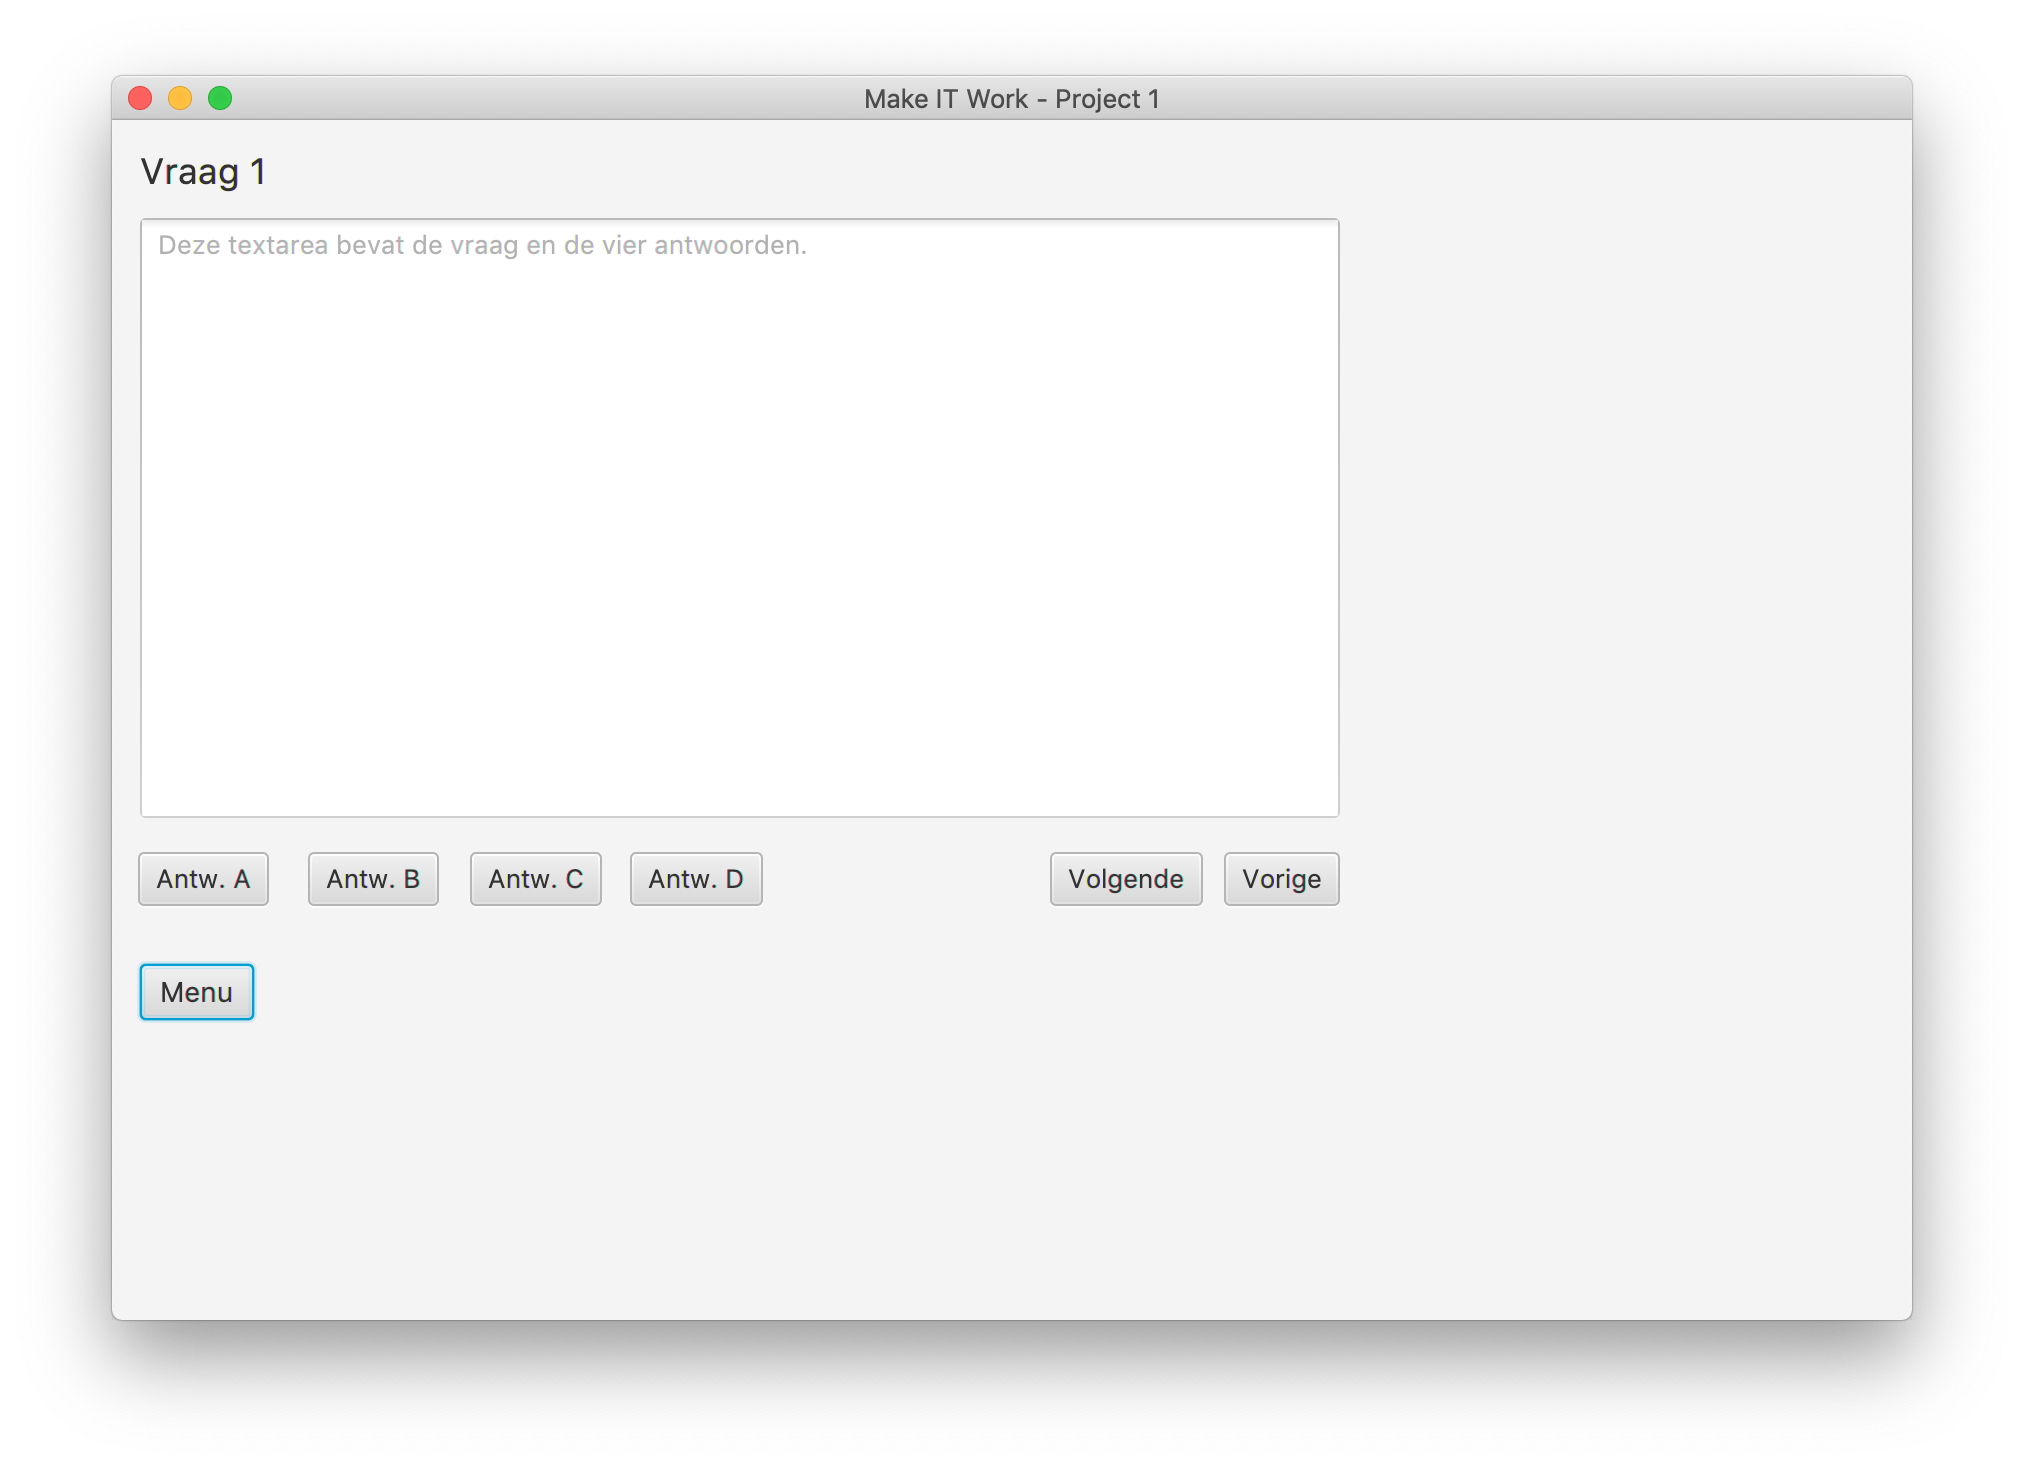
\includegraphics[width=\linewidth]{Screenshot_fillOutQuiz.png}
\end{center}

Hou rekening met het volgende:
\begin{itemize}
\item Het label (``Vraag 1'' in de figuur) moet worden aangepast om het juiste vraagnummer weer te geven.

\item De text area bevat de vraag en de antwoorden.
De antwoorden worden daarbij in willekeurige volgorde gepresenteerd.

\item Door op een van de knoppen Antw. A t/m Antw. C te klikken wordt het betreffende antwoord geregistreerd en de volgende vraag getoond.

\item Door op Volgende te klikken wordt de volgende vraag getoond maar er wordt geen antwoord geregistreerd.

\item Door op Vorige te klikken wordt de vorige vraag getoond zonder een antwoord te registreren.

\item Als een student een vraag twee of meer keer beantwoordt, wordt alleen het laatst gegeven antwoord geregistreerd.

\item Als de laatste vraag is beantwoord, of als de student bij de laatste vraag op Volgende klikt wordt het feedback scherm getoond.

\end{itemize}

\paragraph{Quiz afsluiten en feedback}
Als student wil ik na de beantwoording van de laatste vraag een scherm zien met daarop een overzicht van alle keren dat ik deze quiz heb gedaan met daarbij het behaalde resultaat. (Scherm studentFeedback.fxml)

\subsection{User stories voor de rol Docent}

Functionaliteit voor de docenten behoort niet tot deze release van de applicatie.

\subsection{User stories voor de rol Co\"ordinator}

\paragraph{Dashboard}
Als co\"ordinator wil ik \'e\'en scherm een overzicht kunnen opvragen van alle cursussen, quizen en vragen waarvoor ik de rol co\"ordinator heb.
Dit scherm bevat drie lijsten: een lijst van cursussen, een lijst van quizes voor de geselecteerde cursus en een lijst van vragen voor de geselecteerde quiz.
Als er geen cursus is geselecteerd is de lijst van quizes leeg, en mutatis mutandi geldt dit ook voor de lijst van vragen.
Iedere lijst heeft twee knoppen: een knop om een nieuw item in die lijst te maken en een knop om het geselecteerde item in die lijst te wijzigen.
Merk op dat het maken en wijzigen van cursussen ook al onderdeel is van de functionaliteit van de Onderwijsadministratie\footnote{De CRUD functionaliteit is niet volledig: verwijderen van cursussen/quizes/vragen is hier niet mogelijk. Informeer bij de product owner hoe je hiermee moet omgaan.}!
Het scherm (CoordinatorDashboard.fxml) ziet er zo uit:

\begin{center}
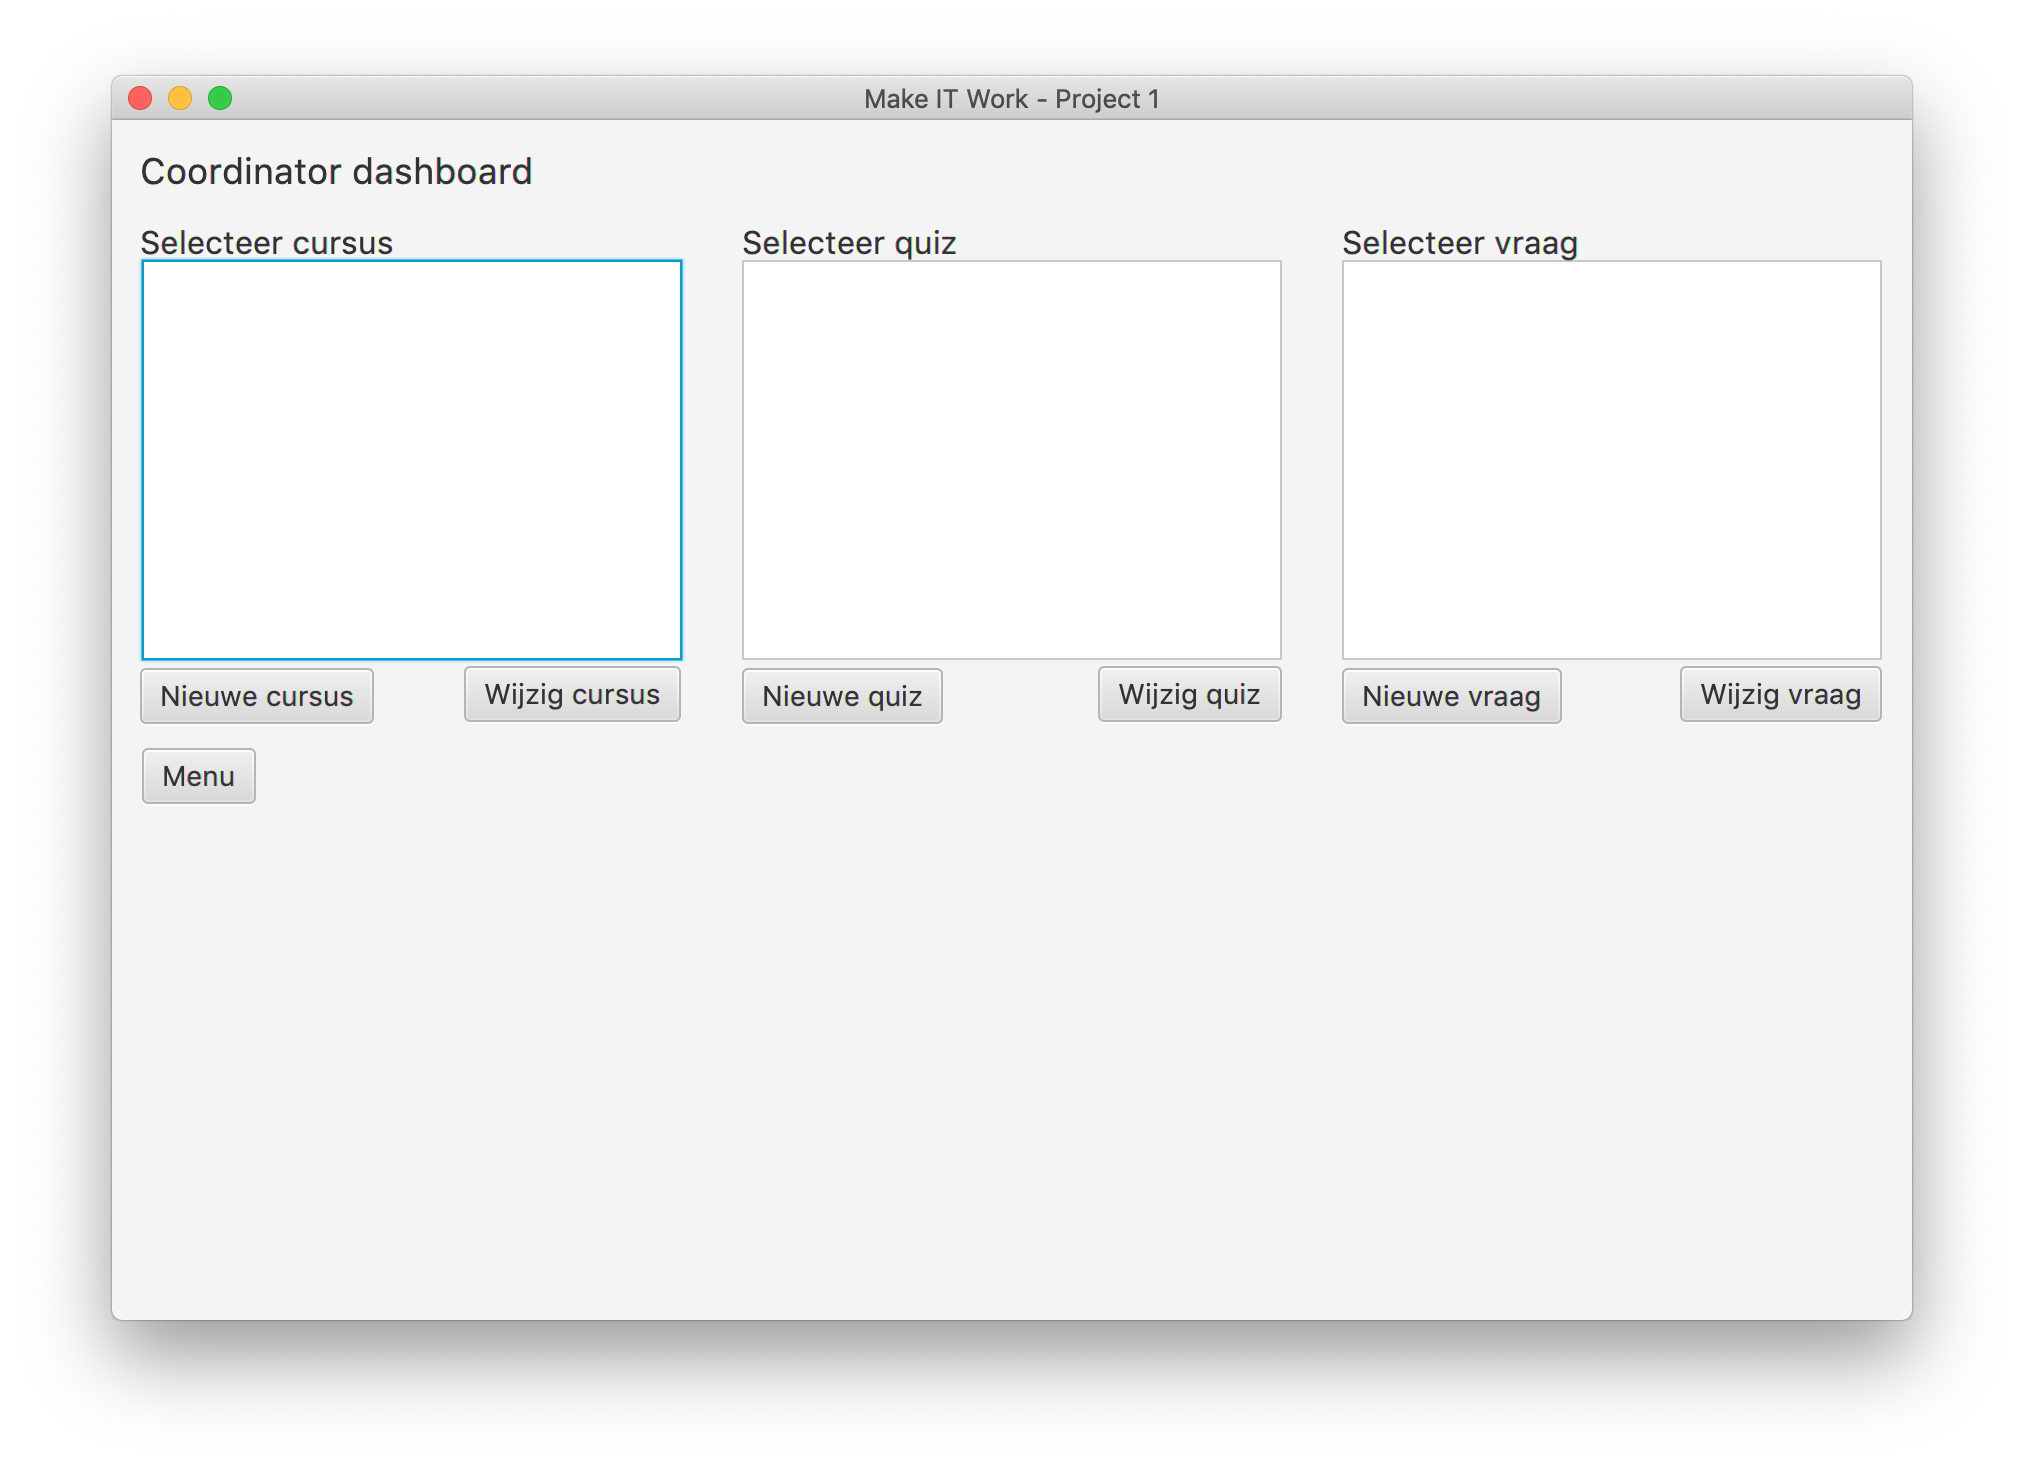
\includegraphics[width=\linewidth]{CoordinatorDashboard.png}
\end{center}

\paragraph{Vragen maken en bewerken}
Als co\"ordinator wil ik een nieuwe vraag kunnen maken.
Een vraag is altijd multiple-choice met vier mogelijke antwoorden.
Daarom wil ik:
\begin{enumerate}
\item De tekst van de vraag invoeren of wijzigen.
\item De tekst van ieder antwoord invoeren of wijzigen.
\item Een bestaand antwoord wijzigen.
\end{enumerate}

\textbf{NB 1!} In de lijst van antwoorden moet het eerste antwoord het juiste zijn.
De volgende antwoorden in de lijst zijn de onjuiste antwoorden.
Bij de presentatie van een vraag aan een student worden de antwoorden in een willekeurige volgorde aangeboden zodat het eerste niet noodzakelijkerwijs het juiste is. (Scherm newQuestion.fxml)

\textbf{NB 2!} Voor het maken van nieuwe vragen en het bewerken van bestaande moet hetzelfde scherm worden gebruikt (newQuestion.fxml).
Bij nieuwe vragen is dist scherm leeg, bij het bewerken van bestaande vragen wordt de inhoud van de vraag getoond.

\textbf{NB 3!} Selectie van de te maken of bewerken vraag gaat altijd via het co\"ordinator dashboard.

\subsection{User stories voor de rol Administrator}

\paragraph{Cursus CRUD}
Als administrator wil ik de volledige crud-functionaliteit voor het beheer van cursussen hebben. (schermen manageCourses.fxml, changeCourse.fxml, newCourse.fxml).

\paragraph{Groepen CRUD}
Als administrator wil ik de volledige crud-functionaliteit voor het beheer van groepen hebben. Toevoegen en verwijderen van studenten aan groepen hoort hier nog niet bij (deze functionaliteit is geen onderdeel van de huidige release)! (schermen manageGroups.fxml, changeGroup.fxml, newGroup.fxml).

\subsection{User stories voor de rol Technisch beheerder}

\paragraph{Overzicht gebruikers} Als technisch beheerder wil ik een overzicht kunnen zien van alle geregistreerde gebruikers. (scherm selectUser.fxml)

\paragraph{Gebruiker aanmaken} Als technisch beheerder wil ik een nieuwe gebruiker aanmaken en daarbij zijn rol vastleggen zodat deze gebruiker toegang tot het systeem kan krijgen. (scherm newUser.fxml)

\paragraph{Gebruiker wijzigen} Als technisch beheerder wil ik de gegevens van een bestaande gebruiker wijzigen zodat de gegevensadministratie up-to-date blijft. (scherm changeUser.fxml)

\paragraph{Gebruiker verwijderen} Als technisch beheerder wil ik een bestaande gebruiker verwijderen om te voorkomen dat gebruikers onterecht toegang tot het systeem houden. (scherm deleteUser.fxml)

\end{document}